% 2011 年四川卷理科第 19 题：直三棱柱 ABC-A1B1C1，D 在棱 CC1 上，
%   P 为 AD 的延长线与 A1C1 的延长线的交点，且 PB1∥平面 BDA1。
% 来源 PDF：普通高考/2011/2011四川理.pdf，SHA-256 116ce515679869425079ef4777505df3735ba4cba64847c9069b7d7acdb4fda4。
% 原页：第 2 页（A3 三栏）第 1 栏上部，书页码 702。
% 重绘依据：照原页——顶面 ABC 可见，B 在左、A 在上、C 在右上；B1 在左下（前面的竖棱 BB1 实线），
%   A1 为被遮挡的顶点（AA1 虚线），C1 在 D 的正下方；D 在 CC1 中点；
%   P 在 A1C1 延长线上（C1 之外），AD 的延长线过 D 到 P。
%   实线：AB、AC、BC、BB1、CC1、BD、B1D、B1P、DP；
%   虚线：AA1、A1B1、A1C1 及其延长至 P、B1C1、BA1、AD。
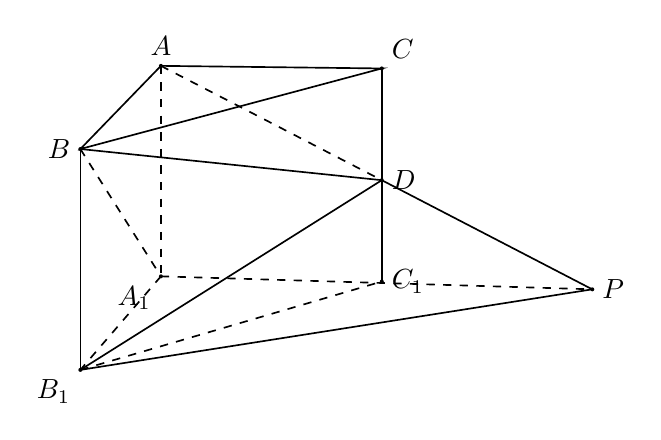
\begin{tikzpicture}[scale=0.66, >=stealth, semithick]
  \coordinate (A)  at (3.10,6.60);
  \coordinate (B)  at (1.55,5.00);
  \coordinate (C)  at (7.35,6.55);
  \coordinate (A1) at (3.10,2.55);
  \coordinate (B1) at (1.55,0.75);
  \coordinate (C1) at (7.35,2.45);
  \coordinate (D)  at (7.35,4.40);
  \coordinate (P)  at (11.40,2.30);

  % 可见棱（实线）
  \draw (A) -- (B) -- (C) -- cycle;
  \draw (B) -- (B1);
  \draw (C) -- (C1);
  \draw (B) -- (D);
  \draw (B1) -- (D);
  \draw (B1) -- (P);
  \draw (D) -- (P);

  % 被遮挡的棱（虚线）
  \draw[dashed] (A) -- (A1);
  \draw[dashed] (A1) -- (B1);
  \draw[dashed] (A1) -- (P);
  \draw[dashed] (B1) -- (C1);
  \draw[dashed] (B) -- (A1);
  \draw[dashed] (A) -- (D);

  \fill (A) circle (1.1pt);
  \fill (B) circle (1.1pt);
  \fill (C) circle (1.1pt);
  \fill (A1) circle (1.1pt);
  \fill (B1) circle (1.1pt);
  \fill (C1) circle (1.1pt);
  \fill (D) circle (1.1pt);
  \fill (P) circle (1.1pt);

  \node at (A)  [above] {$A$};
  \node at (B)  [left] {$B$};
  \node at (C)  [above right] {$C$};
  \node at (A1) [below left] {$A_1$};
  \node at (B1) [below left] {$B_1$};
  \node at (C1) [right] {$C_1$};
  \node at (D)  [right] {$D$};
  \node at (P)  [right] {$P$};
\end{tikzpicture}
